\documentclass[12pt,a4paper]{report}

% ------------------------------------------------
% PACKAGES
% ------------------------------------------------
\usepackage[utf8]{inputenc}
\usepackage[T1]{fontenc}
\usepackage[table]{xcolor}
\usepackage{geometry}
\usepackage{graphicx}
\usepackage{float}
\usepackage{array}
\usepackage{tabularx}
\usepackage{booktabs}
\usepackage{longtable}
\usepackage{multirow}
\usepackage{tikz}
\usepackage{pgfplots}
\usepackage[most]{tcolorbox}
\usepackage{fancyhdr}
\usepackage{titlesec}
\usepackage{setspace}
\usepackage{hyperref}
\usepackage{enumitem}
\usepackage{pifont}
\usepackage{microtype}
\usepackage{pgf}

\pgfdeclarelayer{background}
\pgfdeclarelayer{main}
\pgfsetlayers{background,main}

\usetikzlibrary{arrows.meta, positioning, shapes.geometric, shapes.misc}
\pgfplotsset{compat=1.18}

% ------------------------------------------------
% PAGE SETUP
% ------------------------------------------------
\geometry{margin=1in}
\setlength{\headheight}{14.5pt} % Fixed fancyhdr warning
\onehalfspacing
\setlength{\parindent}{0pt}
\setlength{\parskip}{6pt}

% ------------------------------------------------
% COLOR THEME
% ------------------------------------------------
\definecolor{primary}{HTML}{4B2E83}
\definecolor{secondary}{HTML}{EDE7F6}
\definecolor{accent}{HTML}{00897B}
\definecolor{softteal}{HTML}{E0F2F1}
\definecolor{softcream}{HTML}{FFF8E1}
\definecolor{softrose}{HTML}{FCE4EC}
\definecolor{softgray}{HTML}{F5F5F5}
\definecolor{darkgray}{HTML}{333333}
\definecolor{nextstepblue}{HTML}{005BB5} % Vibrant Corporate Blue for Cover

% ------------------------------------------------
% HYPERLINK SETUP
% Contents, List of Figures, and List of Tables are black
% ------------------------------------------------
\hypersetup{
    colorlinks=true,
    linkcolor=black,
    urlcolor=black,
    citecolor=black
}

% ------------------------------------------------
% HEADER AND FOOTER
% ------------------------------------------------
\pagestyle{fancy}
\fancyhf{}
\fancyhead[L]{Information System Analysis Report}
\fancyhead[R]{}
\fancyfoot[C]{\thepage}
\renewcommand{\headrulewidth}{0.4pt}

% ------------------------------------------------
% TITLE FORMATTING
% ------------------------------------------------
\titleformat{\chapter}
  {\normalfont\huge\bfseries\color{primary}}
  {Chapter \thechapter}
  {20pt}
  {}

\titleformat{\section}
  {\normalfont\Large\bfseries\color{primary}}
  {\thesection}
  {1em}
  {}

\titleformat{\subsection}
  {\normalfont\large\bfseries\color{accent}}
  {\thesubsection}
  {1em}
  {}

\titleformat{\subsubsection}
  {\normalfont\normalsize\bfseries\color{primary}}
  {}
  {0pt}
  {}

% ------------------------------------------------
% CUSTOM BOXES
% ------------------------------------------------
\newtcolorbox{highlightBox}{
    enhanced,
    colback=secondary,
    colframe=primary,
    boxrule=1pt,
    arc=1mm,
    left=9pt,
    right=9pt,
    top=9pt,
    bottom=9pt,
    borderline west={4pt}{0pt}{primary}
}

\newtcolorbox{problemBox}{
    enhanced,
    colback=softrose,
    colframe=primary!80!black,
    boxrule=1pt,
    arc=1mm,
    left=9pt,
    right=9pt,
    top=9pt,
    bottom=9pt,
    fonttitle=\bfseries,
    title=\textbf{Problem Statement},
    borderline west={4pt}{0pt}{primary!80!black}
}

\newtcolorbox{summaryBox}{
    enhanced,
    colback=softteal,
    colframe=accent,
    boxrule=1pt,
    arc=1mm,
    left=9pt,
    right=9pt,
    top=9pt,
    bottom=9pt,
    fonttitle=\bfseries,
    title=\textbf{Feasibility Summary},
    borderline west={4pt}{0pt}{accent}
}

\newtcolorbox{recommendBox}{
    enhanced,
    colback=softcream,
    colframe=orange!80!black,
    boxrule=1.3pt,
    arc=1mm,
    left=11pt,
    right=11pt,
    top=12pt,
    bottom=10pt,
    fonttitle=\bfseries\large,
    title=\textbf{\ding{72} Recommended Action},
    attach boxed title to top left={xshift=5mm,yshift=-2mm},
    boxed title style={
        colback=orange!80!black,
        colframe=orange!80!black,
        coltext=white,
        arc=1mm
    },
    borderline west={5pt}{0pt}{orange!80!black}
}

\newtcolorbox{noteBox}{
    enhanced,
    colback=softgray,
    colframe=primary,
    boxrule=1pt,
    arc=1mm,
    left=9pt,
    right=9pt,
    top=9pt,
    bottom=9pt,
    borderline west={4pt}{0pt}{primary}
}

% ------------------------------------------------
% DOCUMENT START
% ------------------------------------------------
\begin{document}

% ------------------------------------------------
% TITLE PAGE
% ------------------------------------------------
\begin{titlepage}
    \centering
    \vspace*{0.5cm}

    % University Logo & Name
    
\includegraphics[width=0.2\textwidth]{ruet_logo.png}\\[0.4cm]
    {\LARGE \textbf{Rajshahi University of Engineering \& Technology}}\\[1.5cm]

    % Report Titles & Horizontal Rules for Professional Look
    {\color{nextstepblue}\rule{\textwidth}{2pt}}\\[0.8cm]
    {\Huge \textbf{NextStepBD}}\\[0.5cm]
    {\Large \textbf{Information System Analysis and Design Report}}\\[0.8cm]
    {\Large \textbf{Course Title:} Information System Analysis and Design Sessional}\\[0.3cm]
    {\large \textbf{Course Code:} CSE 4110}\\[0.6cm]
    {\color{nextstepblue}\rule{\textwidth}{2pt}}\\[2.5cm]

    % Two-column layout using tabularx format
    \large
    \begin{tabularx}{\textwidth}{@{} >{\raggedright\arraybackslash}X >{\raggedleft\arraybackslash}X @{}}
        {\Large \textcolor{nextstepblue}{\textbf{Submitted By:}}} & {\Large \textcolor{nextstepblue}{\textbf{Submitted To:}}} \\[0.4cm]
        Mst. Mim Afsana Mim (\textit{2103043}) & \textbf{Dr. Md. Rabiul Islam} \\
        Md. Naimuzzaman (\textit{2103044}) & Professor \\
        Arpita Karmokar (\textit{2103045}) & Dept. of Computer Science \& \\
        Md Shehab Sarker (\textit{2103046}) & Engineering \\
        & Rajshahi University of Engineering \& Technology \\
         \\
    \end{tabularx}

    \vfill
\end{titlepage}

\tableofcontents
\listoffigures
\listoftables
\newpage

% ================================================================
% CHAPTER 1
% ================================================================
\chapter{Recognition of Need}

\section{Introduction}

NextStepBD is a Bangladesh-based technology company that provides software development, automation solutions, and consultancy services. The company focuses on building customized digital solutions for local and international clients. Its work environment is fast-moving and client-driven, where quick communication, flexible decision-making, and rapid project execution are important for daily operations.

The company provides both product-based and service-based solutions. Its product development activities include standalone software systems such as doctor management systems, AI-based customer support platforms, and sales automation tools. Alongside software development, NextStepBD also provides consultancy services for internal workflow automation. One notable example is an automation solution where sales data collected through SMS was entered into a centralized software system for analytics, inventory tracking, and supply chain reporting.

\begin{highlightBox}
\textbf{Recognition of Need:} NextStepBD has a functional working system, but the system is not fully centralized. The company uses several separate tools for communication, development, reporting, and coordination. This creates a need for a more integrated information system that can support future growth.
\end{highlightBox}

The company currently relies on a combination of custom-built tools and commonly used platforms such as Microsoft Excel, Google Sheets, GitHub, WhatsApp, Slack, and Email. These tools are useful individually, but they are not connected through a single system. As a result, managers and employees often need to coordinate manually, transfer information between platforms, and search through different communication channels to find project-related information.

\section{Company Overview}

NextStepBD operates as an IT-based software and automation company. Its business model is based on delivering customized digital solutions according to client needs. The company works with software systems, AI-based tools, workflow automation, and customer support solutions. This makes the organization dependent on accurate requirement collection, strong coordination between teams, proper task assignment, and reliable communication with clients.

The organizational structure of NextStepBD is relatively flat. This helps the company make decisions quickly and respond to client requests faster. However, the same structure also creates dependency on a limited number of managers or coordinators. These individuals often act as the bridge between clients and developers. If proper documentation and task tracking systems are not maintained, the workflow can become unclear and difficult to scale.

\begin{table}[H]
\centering
\renewcommand{\arraystretch}{1.3}
\begin{tabularx}{\textwidth}{|p{4cm}|X|}
\hline
\rowcolor{secondary}
\textbf{Area} & \textbf{Description} \\
\hline
Company Name & NextStepBD \\
\hline
Business Type & IT-based software development, automation, and consultancy company \\
\hline
Core Activities & Customized software development, workflow automation, AI-based support tools, sales automation, and reporting solutions \\
\hline
Working Style & Client-driven, flexible, fast communication-based, and semi-structured \\
\hline
Current Operational Approach & Uses multiple separate tools for communication, development, reporting, and coordination \\
\hline
Major Need & A centralized and integrated information system to improve coordination, tracking, reporting, and scalability \\
\hline
\end{tabularx}
\caption{NextStepBD -- Organizational Profile}
\end{table}

\section{Business Activities and Service Context}

NextStepBD serves clients by designing and developing software systems that solve practical business problems. The company’s services can be understood through three major areas: software development, automation consultancy, and customer support solutions.

In software development, the company builds standalone systems based on client requirements. These systems may include management software, operational software, or business-specific applications. In automation consultancy, NextStepBD helps organizations reduce manual work by designing automated workflows. For example, sales data collection through SMS and automatic entry into a reporting system shows how the company uses technology to improve business efficiency. In customer support solutions, the company helps businesses manage social media communication and client interactions more effectively.

These activities require continuous communication between clients, managers, and developers. Requirements must be collected clearly, tasks must be assigned properly, progress must be tracked, and reports must be prepared accurately. Therefore, the quality of the company’s internal information system directly affects project delivery and client satisfaction.

\section{Existing System and Tools Used}

The current system of NextStepBD is not based on one centralized platform. Instead, it is formed by a combination of several digital tools. WhatsApp is heavily used for fast communication with clients and internal teams. Slack is used mainly for more structured or international collaboration. Email is used for formal communication and final reporting. GitHub supports development and version control. Excel and Google Sheets are used for reporting, data management, financial records, and client-side collaboration.

This tool-based system gives flexibility, but it also creates fragmentation. Information about the same project may exist in WhatsApp messages, Google Sheets, GitHub repositories, and email threads. A manager may need to check multiple platforms to understand the actual progress of a project. Similarly, developers may receive instructions from chat messages while technical updates are maintained in GitHub. This separation creates a gap between communication and execution.

\begin{table}[H]
\centering
\renewcommand{\arraystretch}{1.3}
\begin{tabularx}{\textwidth}{|p{4cm}|X|}
\hline
\rowcolor{secondary}
\textbf{Tool / Platform} & \textbf{Operational Role} \\
\hline
WhatsApp & Used for quick client communication, internal coordination, informal discussions, and urgent updates. \\
\hline
Slack & Used for structured team communication and international collaboration in selected cases. \\
\hline
Email & Used for formal communication, official document sharing, and final report delivery. \\
\hline
GitHub & Used for source code management, version control, and developer collaboration. \\
\hline
Microsoft Excel and Google Sheets & Used for reporting, financial records, shared data handling, and client-side collaboration. \\
\hline
Custom Tools & Used for automation, data processing, analytics, and workflow support in specific projects. \\
\hline
\end{tabularx}
\caption{Current Tools and Their Operational Role}
\end{table}

\begin{figure}[H]
\centering
\resizebox{0.95\textwidth}{!}{
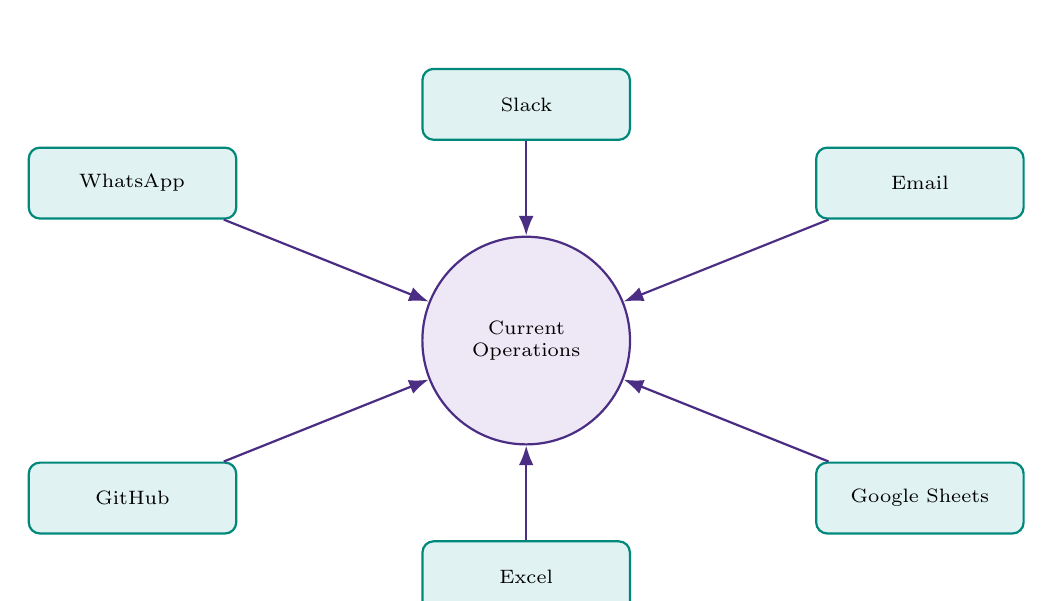
\begin{tikzpicture}[
    every node/.style={font=\scriptsize},
    tool/.style={
        rectangle,
        rounded corners,
        draw=accent,
        fill=softteal,
        thick,
        text width=2.4cm,
        minimum height=0.9cm,
        align=center
    },
    center/.style={
        circle,
        draw=primary,
        fill=secondary,
        thick,
        text width=2.3cm,
        minimum size=2.4cm,
        align=center
    },
    arrow/.style={thick, -{Latex[length=2.5mm]}, color=primary}
]

\node[center] (ops) at (0,0) {Current\\Operations};

\node[tool] (wa) at (-5,2) {WhatsApp};
\node[tool] (slack) at (0,3) {Slack};
\node[tool] (email) at (5,2) {Email};
\node[tool] (github) at (-5,-2) {GitHub};
\node[tool] (excel) at (0,-3) {Excel};
\node[tool] (sheets) at (5,-2) {Google Sheets};

\draw[arrow] (wa) -- (ops);
\draw[arrow] (slack) -- (ops);
\draw[arrow] (email) -- (ops);
\draw[arrow] (github) -- (ops);
\draw[arrow] (excel) -- (ops);
\draw[arrow] (sheets) -- (ops);

\end{tikzpicture}
}
\caption{Current Tool-Based Operational Environment}
\end{figure}

\section{Current Workflow}

The current workflow of NextStepBD begins when a client communicates requirements through WhatsApp, shared documents, Google Sheets, or email. The manager reviews the requirement and assigns tasks to developers. Developers then work on the assigned task using GitHub for version control. During development, internal communication takes place mainly through WhatsApp groups or direct messages. After the work is completed, reports are prepared using Excel or Google Sheets and delivered to the client through email or shared links.

This workflow is practical for a small team and allows quick communication. However, it becomes less effective as the number of projects, clients, and developers increases. Since the workflow depends on manual coordination, project information can become scattered. For example, the client’s requirement may be in WhatsApp, task progress may be in GitHub, and final reporting may be in Google Sheets. Without a centralized system, it becomes difficult to maintain a single source of truth.

\begin{figure}[H]
\centering
\resizebox{\textwidth}{!}{
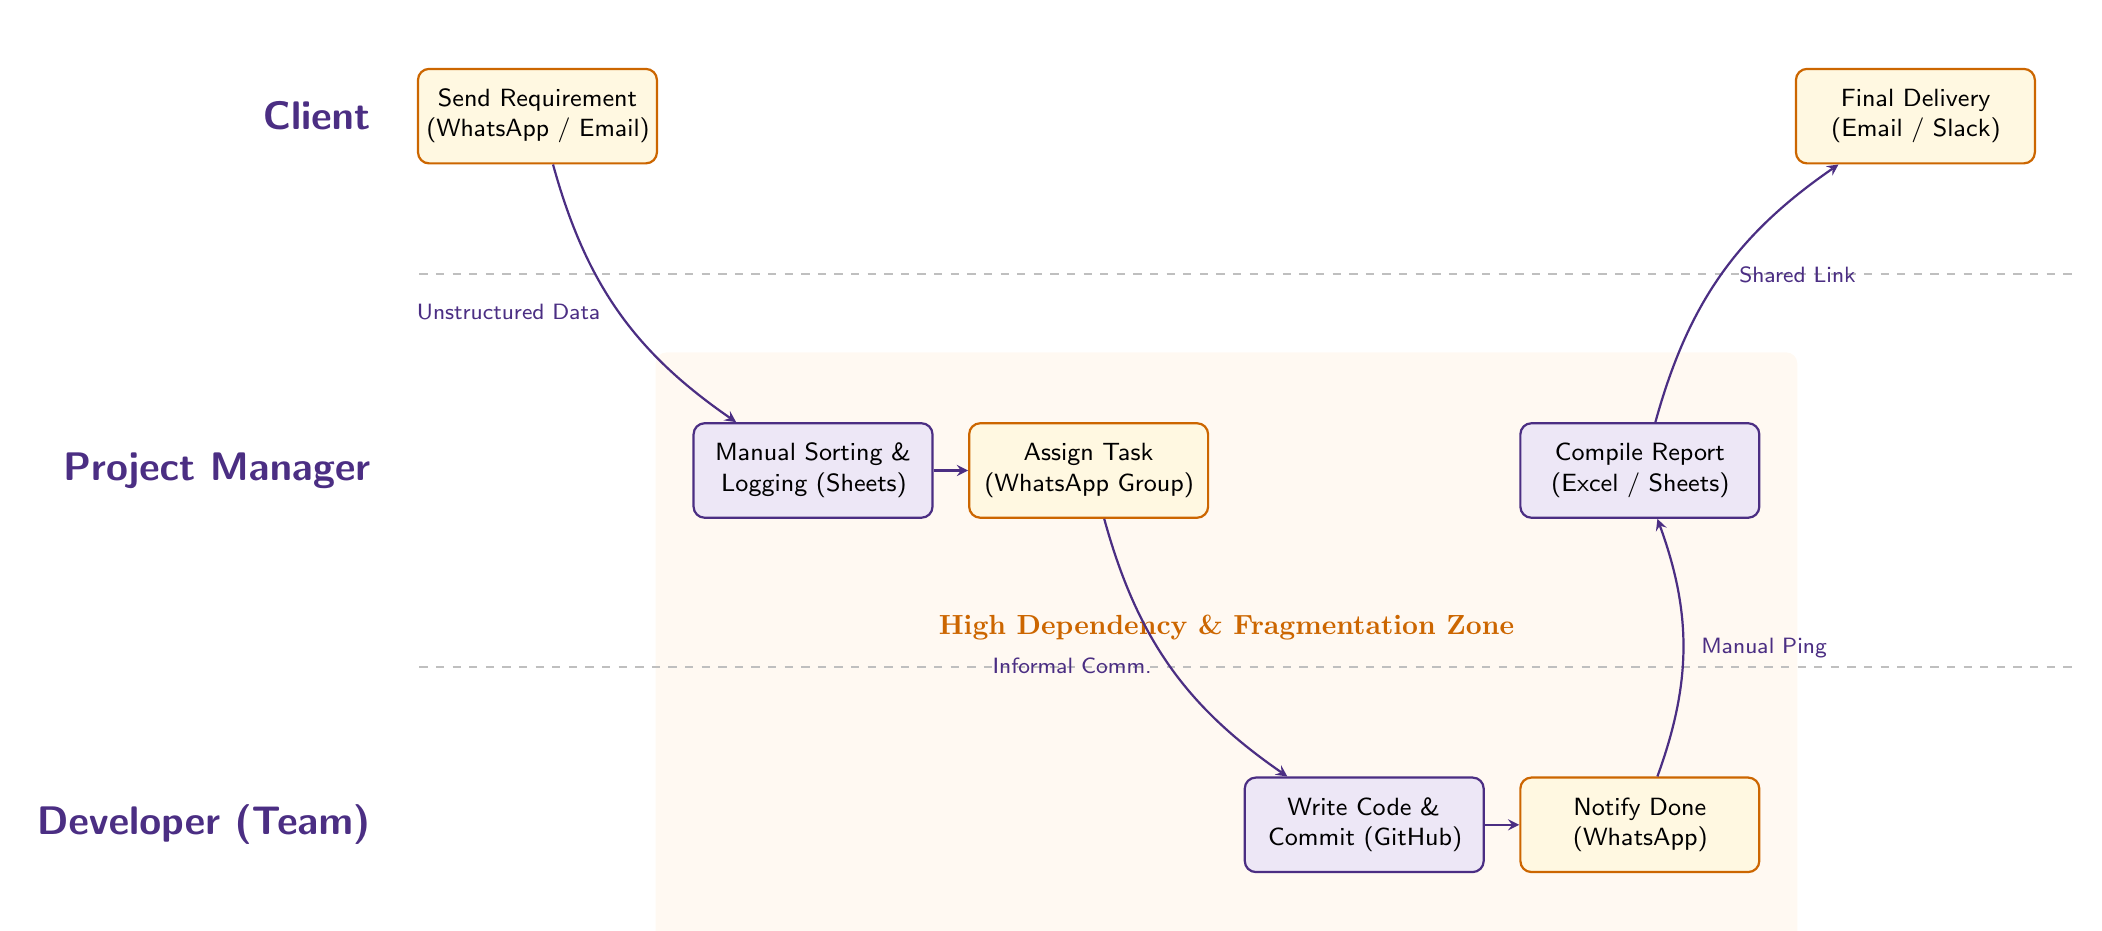
\begin{tikzpicture}[
    every node/.style={font=\sffamily\small},
    swimlane/.style={draw=gray!50, dashed, thick},
    box/.style={
        rectangle, 
        rounded corners, 
        draw=primary, 
        fill=secondary, 
        thick, 
        text width=2.8cm, 
        align=center, 
        minimum height=1.2cm
    },
    riskbox/.style={
        rectangle, 
        rounded corners, 
        draw=orange!80!black, 
        fill=softcream, 
        thick, 
        text width=2.8cm, 
        align=center, 
        minimum height=1.2cm
    },
    arrow/.style={->, >=stealth, thick, color=primary},
    labelnode/.style={font=\sffamily\Large\bfseries, color=primary}
]

% SWIMLANES
\draw[swimlane] (0,2.5) -- (21,2.5);
\draw[swimlane] (0,-2.5) -- (21,-2.5);

% LANE LABELS
\node[labelnode, left] at (-0.5, 4.5) {Client};
\node[labelnode, left] at (-0.5, 0) {Project Manager};
\node[labelnode, left] at (-0.5, -4.5) {Developer (Team)};

% NODES
\node[riskbox] (req) at (1.5, 4.5) {Send Requirement\\(WhatsApp / Email)};
\node[box] (log) at (5.0, 0) {Manual Sorting \&\\Logging (Sheets)};
\node[riskbox] (assign) at (8.5, 0) {Assign Task\\(WhatsApp Group)};
\node[box] (code) at (12.0, -4.5) {Write Code \&\\Commit (GitHub)};
\node[riskbox] (notify) at (15.5, -4.5) {Notify Done\\(WhatsApp)};
\node[box] (report) at (15.5, 0) {Compile Report\\(Excel / Sheets)};
\node[riskbox] (delivery) at (19.0, 4.5) {Final Delivery\\(Email / Slack)};

% ARROWS
\draw[arrow] (req) edge[bend right=20] node[left, xshift=-0.1cm] {\footnotesize Unstructured Data} (log);
\draw[arrow] (log) -- (assign);
\draw[arrow] (assign) edge[bend right=20] node[left, xshift=-0.1cm] {\footnotesize Informal Comm.} (code);
\draw[arrow] (code) -- (notify);
\draw[arrow] (notify) edge[bend right=20] node[right, xshift=0.1cm] {\footnotesize Manual Ping} (report);
\draw[arrow] (report) edge[bend left=20] node[right, xshift=0.1cm] {\footnotesize Shared Link} (delivery);

% BACKGROUND HIGHLIGHT FOR RISK AREA
\begin{pgfonlayer}{background}
    \fill[orange!5, rounded corners] (3.0, 1.5) rectangle (17.5, -6);
    \node[orange!80!black, font=\bfseries] at (10.25, -2.00) {High Dependency \& Fragmentation Zone};
\end{pgfonlayer}

\end{tikzpicture}
}
\caption{Current Operational Swimlane Diagram Showing the PM Bottleneck}
\end{figure}

\begin{highlightBox}
\textbf{System Observation:} The existing workflow works, but it is heavily dependent on manual communication. The system lacks a centralized dashboard where requirements, tasks, development progress, reports, and decisions can be tracked together.
\end{highlightBox}

\section{Need for System Improvement}

The main need for improvement comes from the gap between the company’s growing operational requirements and its current semi-structured information system. As NextStepBD handles more clients and more development tasks, the existing tool-based workflow may become difficult to manage. Manual coordination can slow down decision-making, increase dependency on managers, and create confusion among developers.

A modern information system should not only store data but also connect people, processes, and tools. For NextStepBD, this means the improved system should connect client requirements, task assignment, developer work, communication history, reporting data, and project status. Such a system would help managers monitor progress, developers understand priorities, and clients receive more structured updates.

The need is therefore not simply to introduce new software. The actual need is to create a more organized and integrated work environment where every project has clear requirements, assigned tasks, documented communication, visible progress, and reliable reporting.

\section{Problem Identification}

Through observation of the company’s operations, informal interviews with team members, and an analysis of the current workflow, five major problem areas have been identified. These act as the core constraints to the organization's scalability and stability, ordered below by their severity.

\subsection{Problem 01: Fragmented System Architecture and Lack of Integration}

\begin{problemBox}
NextStepBD uses multiple disconnected platforms such as WhatsApp, Google Sheets, GitHub, Slack, and Email. There is no centralized system connecting communication, development, and tracking.
\end{problemBox}

The foundational issue is the absence of connection between these tools. Code is managed in GitHub, communication is lost in WhatsApp, and tasks are manually updated in Sheets. This lack of integration leads to poor traceability, disconnected version control, hidden knowledge, and inefficient reporting.

\subsection{Problem 02: The Project Manager Bottleneck and Central Dependency}

\begin{problemBox}
Project Managers act as the single communication bridge between clients and developers. If a manager is unavailable, the entire development pipeline stalls.
\end{problemBox}

Because task assignment and requirement interpretations are strictly relayed by the Project Manager, they become a single point of failure. This creates deep knowledge silos. Developers lack a direct source of truth for the project, leading to work stoppages whenever a central coordinator becomes overloaded.

\subsection{Problem 03: Unstructured Requirement Gathering and Scope Creep}

\begin{problemBox}
Client requirements are frequently accepted via informal WhatsApp messages without standard documentation. This results in shifting expectations and mid-development changes.
\end{problemBox}

Treating chat messages as formal software requirements creates ambiguity. Developers are forced to make assumptions, causing a mismatch between client expectations and the final product. The lack of standard SRS (Software Requirement Specifications) leads to endless rework, missed deadlines, and timeline overruns.

\subsection{Problem 04: Absence of a Centralized Task Tracking System}

\begin{problemBox}
There is no dedicated software to track who is working on what, when tasks are due, or how much time a specific feature actually took to build.
\end{problemBox}

Without a source of truth for task progress, developers guess their priorities. Furthermore, management has zero visibility into actual team bandwidth. It is virtually impossible to compare estimated development time with actual time taken, making resource planning highly inefficient.

\subsection{Problem 05: Quality Assurance and Deployment Vulnerabilities}

\begin{problemBox}
The technical pipeline lacks modern software engineering safeguards. Developers test their own code informally, and deployments to production are performed manually.
\end{problemBox}

Without a dedicated Quality Assurance (QA) process or automated test workflows, the risk of pushing bugs to clients is unsustainably high. Additionally, manual deployments lack the safety of a CI/CD pipeline, increasing the risk of human error during releases and posing a direct threat to client trust.

\section{Problem Severity Overview}

The following graph shows the estimated severity level of the identified problems based on their impact on operations, stability, and scalability.

\begin{figure}[H]
\centering
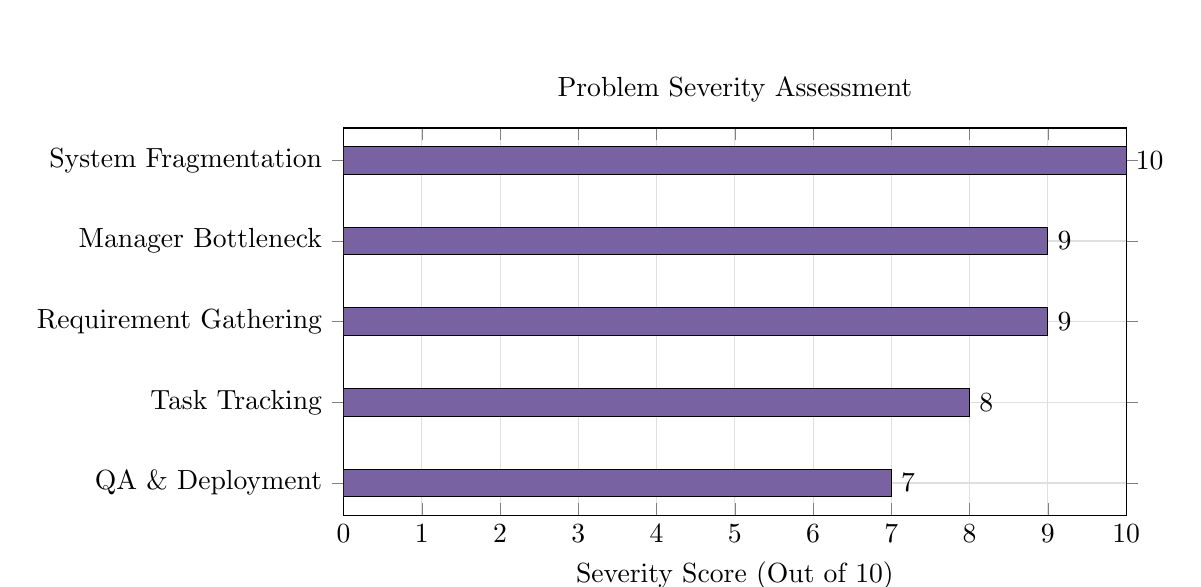
\begin{tikzpicture}
\begin{axis}[
    xbar,
    width=0.95\textwidth,
    height=6.5cm,
    xmin=0,
    xmax=10,
    xlabel={Severity Score (Out of 10)},
    symbolic y coords={
        QA \& Deployment,
        Task Tracking,
        Requirement Gathering,
        Manager Bottleneck,
        System Fragmentation
    },
    ytick=data,
    nodes near coords,
    grid=major,
    major grid style={draw=gray!25},
    title={Problem Severity Assessment}
]
\addplot[fill=primary!75] coordinates {
    (7,{QA \& Deployment})
    (8,{Task Tracking})
    (9,{Requirement Gathering})
    (9,{Manager Bottleneck})
    (10,{System Fragmentation})
};
\end{axis}
\end{tikzpicture}
\caption{Estimated Severity of Identified Problems}
\end{figure}

\section{Chapter 1 Conclusion}

The recognition of need shows that NextStepBD has successfully established a functional working system using available digital tools. However, the system lacks the structure, integration, and centralized control required for sustainable growth.

The major challenges include a fragmented system architecture, an unsustainable reliance on project managers, unstructured requirement management, the absence of centralized task tracking, and significant software testing vulnerabilities. These problems compound one another: weak requirement management creates task confusion, the lack of an integrated system enforces the manager bottleneck, and manual processes result in unstable deployments.

Therefore, the company needs an integrated information system that can connect requirement management, task tracking, development workflow, testing, and continuous delivery. Chapter 2 analyzes the feasibility of solving these problems using technical, economic, and operational perspectives.

\newpage

% ================================================================
% CHAPTER 2
% ================================================================
\chapter{Initial Feasibility Study}

\section{Introduction}

This chapter presents an initial feasibility study for the five major problems identified in Chapter 1. The purpose of this chapter is to evaluate whether the proposed improvements are technically possible, economically reasonable, and operationally acceptable for NextStepBD.

The feasibility framework used in this chapter follows the standard \textbf{Technical, Economic, and Operational} model.

\begin{noteBox}
\textbf{Feasibility Focus:} The objective of this chapter is not only to propose solutions, but also to determine which solutions are realistic, affordable, and suitable for NextStepBD's current operational environment.
\end{noteBox}

\begin{table}[H]
\centering
\renewcommand{\arraystretch}{1.3}
\begin{tabularx}{\textwidth}{|p{4cm}|X|}
\hline
\rowcolor{secondary}
\textbf{Feasibility Dimension} & \textbf{Evaluation Question} \\
\hline
\textbf{Technical Feasibility} & Can the proposed solution be implemented using available technology, tools, infrastructure, and technical skills? \\
\hline
\textbf{Economic Feasibility} & Are the expected benefits greater than the cost of implementation, training, operation, and maintenance? \\
\hline
\textbf{Operational Feasibility} & Can the organization realistically adopt and continue using the solution within its existing workflow and culture? \\
\hline
\end{tabularx}
\caption{TEO Feasibility Evaluation Criteria}
\end{table}

\begin{figure}[H]
\centering
\resizebox{\textwidth}{!}{
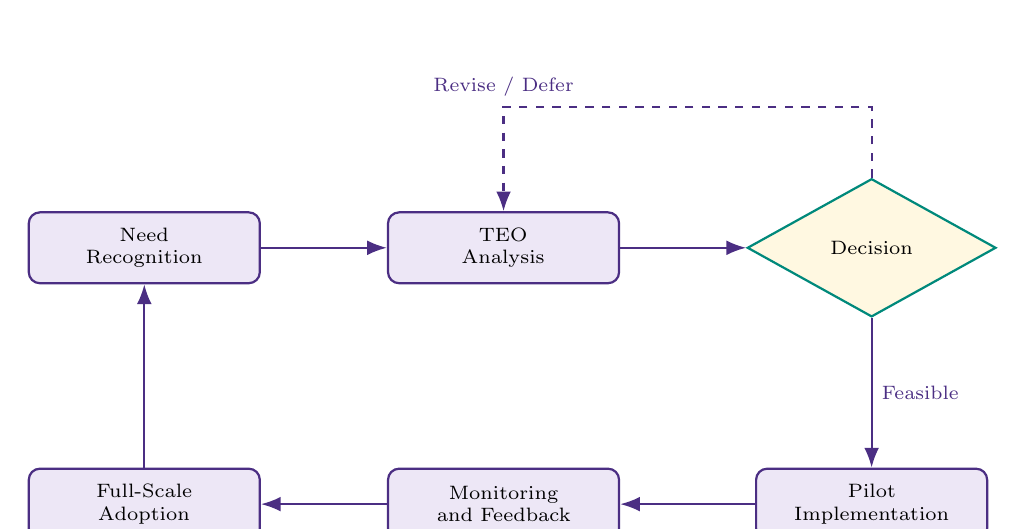
\begin{tikzpicture}[
    node distance=1.6cm,
    every node/.style={font=\scriptsize},
    process/.style={
        rectangle,
        rounded corners,
        draw=primary,
        fill=secondary,
        thick,
        text width=2.7cm,
        minimum height=0.9cm,
        align=center
    },
    decision/.style={
        diamond,
        draw=accent,
        fill=softcream,
        thick,
        aspect=1.8,
        text width=2.2cm,
        align=center
    },
    arrow/.style={thick, -{Latex[length=2.5mm]}, color=primary}
]

\node[process] (need) {Need\\Recognition};
\node[process, right=of need] (analysis) {TEO\\Analysis};
\node[decision, right=of analysis] (decision) {Decision};
\node[process, below=1.9cm of decision] (pilot) {Pilot\\Implementation};
\node[process] (monitor) at (analysis |- pilot) {Monitoring\\and Feedback};
\node[process] (scale) at (need |- pilot) {Full-Scale\\Adoption};

\draw[arrow] (need) -- (analysis);
\draw[arrow] (analysis) -- (decision);
\draw[arrow] (decision) -- node[right, font=\scriptsize]{Feasible} (pilot);
\draw[arrow] (pilot) -- (monitor);
\draw[arrow] (monitor) -- (scale);
\draw[arrow] (scale) -- (need);
\draw[arrow, dashed] (decision.north) -- ++(0,0.9) -| node[above, font=\scriptsize]{Revise / Defer} (analysis.north);

\end{tikzpicture}
}
\caption{Initial Feasibility Governance Cycle for NextStepBD}
\end{figure}

\section{Initial Feasibility Analysis}

\textbf{Baseline Assumptions for Calculations:} NextStepBD is defined as an organization of approximately 50 employees (developers, UI/UX, QA, PMs). Economic feasibility assumes an internal exchange mapping of \$1 USD $\approx$ 120 BDT. All software cost estimations are based on standardized enterprise monthly licensing fees. Employee training costs assume an average internal valuation of \$15/hour per developer.

\subsection{Problem 01: Fragmented System Architecture and Lack of Integration}

\begin{problemBox}
NextStepBD uses multiple disconnected platforms such as WhatsApp, GitHub, Google Sheets, Excel, Slack, and Email. There is no centralized system connecting communication, development, and tracking.
\end{problemBox}

\begin{summaryBox}
An integrated workflow management system is technically feasible because several cloud-based platforms support integration with GitHub, Google Workspace, Slack, and Email. Economically, it can reduce manual work. Operationally, it is suitable if adopted gradually.
\end{summaryBox}

\subsubsection{Details of Findings}

\begin{itemize}[leftmargin=*]
    \item \textbf{Technical Feasibility:} The technical literacy required to adopt Jira Software or Notion is low, as the team already uses digital-first workflows (GitHub, Slack). Integrating Jira via webhooks into Slack and GitHub is a native, out-of-the-box feature requiring no deep API coding.
    \item \textbf{Economic Feasibility:} A Jira Standard license costs \$8.15/user/month. For 50 users, this equals \$4,890 annually (approx. 5.86 Lakh BDT). If the platform saves each employee just 2 hours of manual tracking a month, the ROI (Return on Investment) wildly outweighs the software licensing cost.
    \item \textbf{Operational Feasibility:} Employees already use digital tools, so adoption is realistic. However, strict policy enforcement is needed to stop "shadow IT" (where developers secretly revert to Google Sheets).
    \item \textbf{Risk \& Mitigation:} Change resistance. \textbf{Mitigation:} Phase the rollout. Onboard only the project managers in Month 1, followed by team leads in Month 2.
\end{itemize}

\begin{table}[H]
\centering
\renewcommand{\arraystretch}{1.3}
\begin{tabularx}{\textwidth}{|p{3cm}|p{2.5cm}|X|}
\hline
\rowcolor{secondary}
\textbf{Dimension} & \textbf{Rating} & \textbf{Justification} \\
\hline
Technical & High & Native webhook integration between Jira, Slack, and GitHub requires zero custom development. \\
\hline
Economic & High & Approx. 5.86 Lakh BDT/yr is easily offset by the labor hours saved from chasing status updates. \\
\hline
Operational & Medium & Requires enforcing strict data-entry policies to prevent developers from bypassing the system. \\
\hline
Overall Viability & Feasible & Highly recommended to resolve the foundational problem. \\
\hline
\end{tabularx}
\caption{System Integration -- TEO Feasibility Summary}
\end{table}

\begin{recommendBox}
\textbf{Priority Action:} Adopt a centralized project and workflow management platform across all departments.

\textbf{Business Value:} Eliminates isolated information silos and creates a single reliable source for project data.
\end{recommendBox}

\subsection{Problem 02: The Project Manager Bottleneck and Central Dependency}

\begin{problemBox}
Project Managers act as the single communication bridge. If a manager is unavailable, task assignment stalls, creating a severe operational bottleneck.
\end{problemBox}

\begin{summaryBox}
Relieving the PM bottleneck is highly feasible by shifting from a "push" management style to a transparent "pull" system where developers can view project roadmaps directly.
\end{summaryBox}

\subsubsection{Details of Findings}

\begin{itemize}[leftmargin=*]
    \item \textbf{Technical Feasibility:} Minimal technical hurdles. Setting up a central document repository (like Notion or Confluence Wiki) only requires UI configuration. The infrastructure exists.
    \item \textbf{Economic Feasibility:} High. Notion costs \$10/user/month (10x50x12 = \$6,000/yr or ~7.2 Lakh BDT) but many features are included in Jira (Confluence) bundles. Conversely, GitHub Wiki is entirely free for existing repositories (0 BDT).
    \item \textbf{Operational Feasibility:} High operational friction. Developers must proactively check wikis rather than waiting to be told what to do via WhatsApp. This is a severe cultural shift.
    \item \textbf{Risk \& Mitigation:} Information hoarding. \textbf{Mitigation:} Tie manager KPIs to how effectively they document client requests on the central portal.
\end{itemize}

\begin{table}[H]
\centering
\renewcommand{\arraystretch}{1.3}
\begin{tabularx}{\textwidth}{|p{4cm}|X|X|}
\hline
\rowcolor{secondary}
\textbf{Area} & \textbf{Current State} & \textbf{Proposed State} \\
\hline
Task Discovery & PM manually messages developers & Developers check centralized board \\
\hline
Project Context & Kept in PM's head / WhatsApp & Documented in accessible Wiki \\
\hline
Approval Delays & High when PM is busy & Reduced via peer-review protocols \\
\hline
\end{tabularx}
\caption{Bottleneck Resolution -- Current vs Proposed State}
\end{table}

\begin{recommendBox}
\textbf{Priority Action:} Establish a transparent knowledge base and self-serve task boards.

\textbf{Business Value:} Democratizes project knowledge and speeds up development cycles by removing strict dependencies.
\end{recommendBox}

\subsection{Problem 03: Unstructured Requirement Gathering and Scope Creep}

\begin{problemBox}
Client requirements are accepted via informal WhatsApp messages, leading to mid-development changes, unclear expectations, and heavy rework.
\end{problemBox}

\begin{summaryBox}
Implementing a strict Software Requirement Specification (SRS) intake process is economically near-zero cost and technically simple, though it requires enforcing boundaries with clients.
\end{summaryBox}

\subsubsection{Details of Findings}

\begin{itemize}[leftmargin=*]
    \item \textbf{Technical Feasibility:} Google Forms, internal portals, or Jira issue collectors can standardize requirement intake.
    \item \textbf{Economic Feasibility:} Free to implement using existing platforms.
    \item \textbf{Operational Feasibility:} Will require clients to adjust how they submit requests, demanding PMs to enforce the process.
    \item \textbf{Risk Assessment:} Clients may initially resist filling out forms instead of sending texts.
\end{itemize}

\begin{table}[H]
\centering
\renewcommand{\arraystretch}{1.3}
\begin{tabularx}{\textwidth}{|p{4cm}|X|}
\hline
\rowcolor{secondary}
\textbf{Field} & \textbf{Purpose} \\
\hline
Requirement ID & Provides a unique identification number for tracking. \\
\hline
User Story / Scope & Defines exactly who the feature is for and what it does. \\
\hline
Acceptance Criteria & Defines when the requirement is officially Complete. \\
\hline
Client Sign-off & Formal approval before development begins. \\
\hline
Change Request Delta & Tracks mid-development changes with cost/time implications. \\
\hline
\end{tabularx}
\caption{Proposed Requirement Management Checkpoints}
\end{table}

\begin{recommendBox}
\textbf{Priority Action:} Enforce a standard Software Requirement Specification (SRS) sign-off process before coding starts.

\textbf{Business Value:} Drastically reduces scope creep, stops endless rework loops, and protects profit margins.
\end{recommendBox}

\begin{figure}[H]
\centering
\resizebox{\textwidth}{!}{
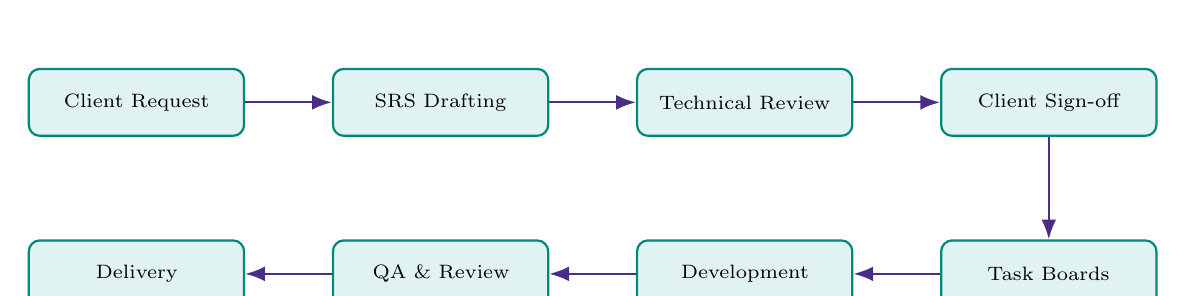
\begin{tikzpicture}[
    node distance=1.1cm,
    every node/.style={font=\scriptsize},
    wf_step/.style={
        rectangle,
        rounded corners,
        draw=accent,
        fill=softteal,
        thick,
        text width=2.5cm,
        minimum height=0.85cm,
        align=center
    },
    arrow/.style={thick, -{Latex[length=2.5mm]}, color=primary}
]

\node[wf_step] (client) {Client Request};
\node[wf_step, right=of client] (template) {SRS Drafting};
\node[wf_step, right=of template] (review) {Technical Review};
\node[wf_step, right=of review] (approve) {Client Sign-off};

\node[wf_step, below=1.3cm of approve] (task) {Task Boards};
\node[wf_step, left=of task] (dev) {Development};
\node[wf_step, left=of dev] (test) {QA \& Review};
\node[wf_step, left=of test] (delivery) {Delivery};

\draw[arrow] (client) -- (template);
\draw[arrow] (template) -- (review);
\draw[arrow] (review) -- (approve);
\draw[arrow] (approve) -- (task);
\draw[arrow] (task) -- (dev);
\draw[arrow] (dev) -- (test);
\draw[arrow] (test) -- (delivery);

\end{tikzpicture}
}
\caption{Proposed Requirement-to-Delivery Workflow}
\end{figure}

\subsection{Problem 04: Absence of a Centralized Task Tracking System}

\begin{problemBox}
Task assignment and project progress tracking are handled manually via chat. There is no single dashboard for tracking deadlines, progress, blockers, or estimated vs. actual development times.
\end{problemBox}

\begin{summaryBox}
A centralized task and project management system is highly feasible. Because developers already use GitHub for version control, project tracking can be embedded directly into their existing environment using GitHub Projects.
\end{summaryBox}

\subsubsection{Details of Findings}

\begin{itemize}[leftmargin=*]
    \item \textbf{Technical Feasibility:} The technical barrier is practically zero. Developers already push code to GitHub. Mapping a pull request (e.g., "Fixes \#42") to an issue card on a GitHub Project board is an automated, native feature.
    \item \textbf{Economic Feasibility:} Free. Instead of purchasing an external project tool, utilizing GitHub Projects is included in the company's existing GitHub base architecture (0 BDT additional cost).
    \item \textbf{Operational Feasibility:} Highly straightforward for developers since it lives inside their IDE ecosystem, but project managers will require a brief 2-hour workshop to learn how to operate an Agile board.
    \item \textbf{Risk \& Mitigation:} The board goes stale. \textbf{Mitigation:} Institute a mandatory 15-minute daily "Stand-up" meeting where the board serves as the only valid metric of progress.
\end{itemize}

\begin{table}[H]
\centering
\renewcommand{\arraystretch}{1.3}
\begin{tabularx}{\textwidth}{|p{3cm}|p{2.5cm}|X|}
\hline
\rowcolor{secondary}
\textbf{Dimension} & \textbf{Rating} & \textbf{Justification} \\
\hline
Technical & High & Native integration with codebase and existing developer accounts requires zero new accounts. \\
\hline
Economic & High & No additional software licensing costs needed (0 BDT). \\
\hline
Operational & High & Smooth developer transition; minimal context switching from code to boards. \\
\hline
Overall Viability & Highly Feasible & Essential for tracking team velocity and output. \\
\hline
\end{tabularx}
\caption{Task Tracking System -- TEO Feasibility Summary}
\end{table}

\begin{recommendBox}
\textbf{Priority Action:} Implement agile task boards (e.g., in GitHub Projects or Jira) with strict limits on "In Progress" work.

\textbf{Business Value:} Provides real-time visibility into team velocity, preventing resource bottlenecks before they happen.
\end{recommendBox}

\subsection{Problem 05: Quality Assurance and Deployment Vulnerabilities}

\begin{problemBox}
Developers test their own code informally without automated testing. Final deployments are done manually, causing a high risk of pushing breaking bugs to live environments.
\end{problemBox}

\begin{summaryBox}
Introducing foundational CI/CD (Continuous Integration/Continuous Deployment) and dedicated peer review is extremely feasible and critical for stabilizing the product lifecycle.
\end{summaryBox}

\subsubsection{Details of Findings}

\begin{itemize}[leftmargin=*]
    \item \textbf{Technical Feasibility:} Moderate challenge. While GitHub Actions scripts are easy to write, the engineering team must learn test-driven methodologies. Training is required to enforce writing unit tests alongside feature arrays.
    \item \textbf{Economic Feasibility:} The cloud infrastructure is cheap. Renting a Virtual Private Server (VPS) via AWS EC2 or DigitalOcean for staging environments costs roughly \$20-\$40/month (~35,000 BDT/yr). The hidden cost is developer time spent writing tests.
    \item \textbf{Operational Feasibility:} Difficult. Developers will initially complain that writing tests "slows them down," clashing with NextStepBD's fast, flexible culture. 
    \item \textbf{Risk \& Mitigation:} Developers bypassing tests. \textbf{Mitigation:} Protect branch merging. Code cannot be merged into the `main` branch unless it passes CI checks and has one verified peer review.
\end{itemize}

\begin{table}[H]
\centering
\renewcommand{\arraystretch}{1.3}
\begin{tabularx}{\textwidth}{|p{5cm}|p{4cm}|X|}
\hline
\rowcolor{secondary}
\textbf{Item} & \textbf{Estimated Annual Cost} & \textbf{Expected Benefit} \\
\hline
CI/CD Infrastructure \& Staging VPS & \$40/mo = \$480/yr ($\approx$57,600 BDT) & Safe environment for clients to test before public release. \\
\hline
Test Engineering Training Hours & 50 devs $\times$ 5 hrs $\times$ \$15/hr ($\approx$4.5 Lakh BDT one-time) & Huge reduction in production bugs; builds technical resilience. \\
\hline
Peer Review Process & Administrative Time & Stops rogue code; enforces coding standards. \\
\hline
\end{tabularx}
\caption{QA and Automation -- Estimated Cost-Benefit Analysis}
\end{table}

\begin{recommendBox}
\textbf{Priority Action:} Mandate peer code reviews for all merges and implement a basic automated deployment pipeline for staging environments.

\textbf{Business Value:} Guarantees product stability, stops regression loops, and significantly boosts client trust.
\end{recommendBox}

\section{Comparative Feasibility Summary}

\begin{table}[H]
\centering
\renewcommand{\arraystretch}{1.3}
\small
\begin{tabularx}{\textwidth}{|c|X|c|c|c|c|c|}
\hline
\rowcolor{secondary}
\textbf{No.} & \textbf{Problem} & \textbf{Tech.} & \textbf{Econ.} & \textbf{Ops.} & \textbf{Est. Cost/yr} & \textbf{Priority} \\
\hline
01 & Fragmented System Architecture and Lack of Integration & H & H & M & BDT 3--8L & Urgent \\
\hline
02 & The Project Manager Bottleneck and Central Dependency & H & H & M & BDT 1--2L & High \\
\hline
03 & Unstructured Requirement Gathering and Scope Creep & H & H & H & BDT 0--1L & Urgent \\
\hline
04 & Absence of a Centralized Task Tracking System & H & H & H & BDT 0--2L & Urgent \\
\hline
05 & Quality Assurance and Deployment Vulnerabilities & H & M & M & BDT 1--3L & High \\
\hline
\end{tabularx}
\caption{Comparative Feasibility Analysis -- Top 5 Core Problems}

\vspace{0.2cm}
\small{\textbf{Note:} H = High, M = Medium. Cost values are approximate annual estimates.}
\end{table}

\begin{figure}[H]
\centering
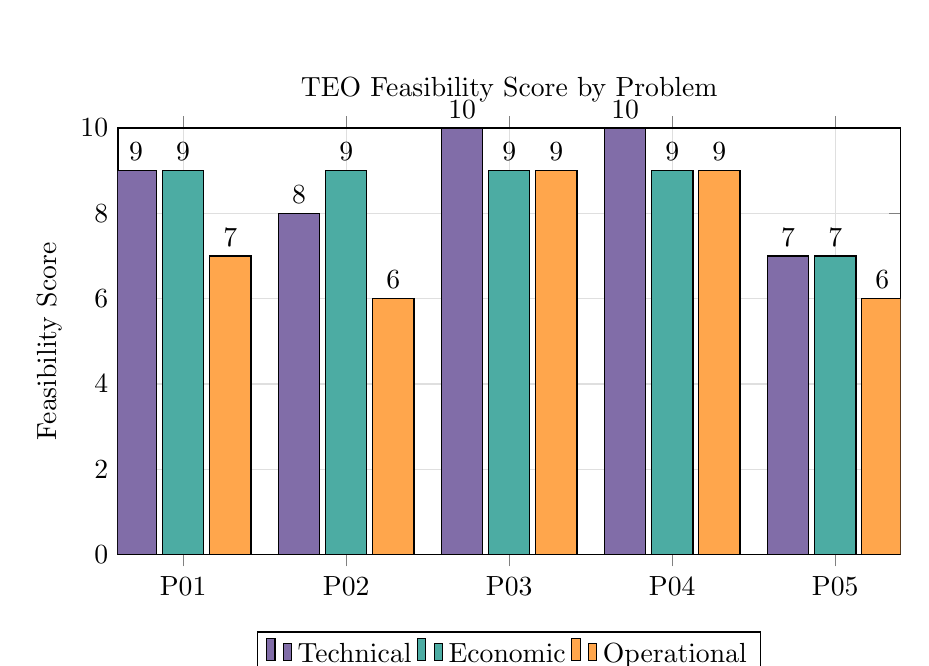
\begin{tikzpicture}
\begin{axis}[
    ybar,
    width=0.95\textwidth,
    height=7cm,
    bar width=15pt,
    ymin=0,
    ymax=10,
    ylabel={Feasibility Score},
    symbolic x coords={P01,P02,P03,P04,P05},
    xtick=data,
    nodes near coords,
    nodes near coords align={vertical},
    legend style={at={(0.5,-0.18)}, anchor=north, legend columns=3},
    grid=major,
    major grid style={draw=gray!25},
    title={TEO Feasibility Score by Problem}
]
\addplot[fill=primary!70] coordinates {(P01,9) (P02,8) (P03,10) (P04,10) (P05,7)};
\addplot[fill=accent!70] coordinates {(P01,9) (P02,9) (P03,9) (P04,9) (P05,7)};
\addplot[fill=orange!70] coordinates {(P01,7) (P02,6) (P03,9) (P04,9) (P05,6)};
\legend{Technical, Economic, Operational}
\end{axis}
\end{tikzpicture}
\caption{Technical, Economic, and Operational Feasibility Comparison}
\end{figure}

\section{Recommended Implementation Roadmap}

\begin{figure}[H]
\centering
\resizebox{\textwidth}{!}{
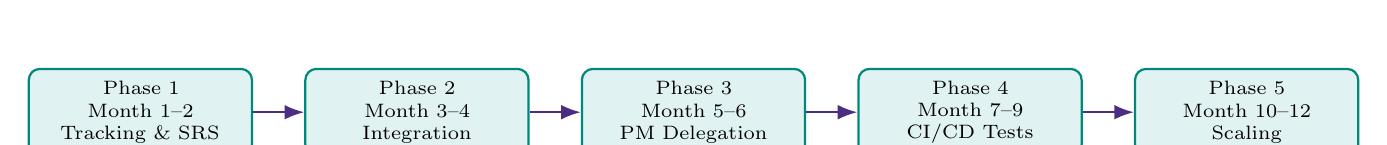
\begin{tikzpicture}[
    node distance=0.65cm,
    every node/.style={font=\scriptsize},
    phase/.style={
        rectangle,
        rounded corners,
        draw=accent,
        fill=softteal,
        thick,
        text width=2.6cm,
        minimum height=1.1cm,
        align=center
    },
    arrow/.style={thick, -{Latex[length=2.5mm]}, color=primary}
]

\node[phase] (ph1) {Phase 1\\Month 1--2\\Tracking \& SRS};
\node[phase, right=of ph1] (ph2) {Phase 2\\Month 3--4\\Integration};
\node[phase, right=of ph2] (ph3) {Phase 3\\Month 5--6\\PM Delegation};
\node[phase, right=of ph3] (ph4) {Phase 4\\Month 7--9\\CI/CD Tests};
\node[phase, right=of ph4] (ph5) {Phase 5\\Month 10--12\\Scaling};

\draw[arrow] (ph1) -- (ph2);
\draw[arrow] (ph2) -- (ph3);
\draw[arrow] (ph3) -- (ph4);
\draw[arrow] (ph4) -- (ph5);

\end{tikzpicture}
}
\caption{Proposed Implementation Roadmap}
\end{figure}

\begin{table}[H]
\centering
\renewcommand{\arraystretch}{1.3}
\begin{tabularx}{\textwidth}{|p{3cm}|X|p{3cm}|}
\hline
\rowcolor{secondary}
\textbf{Phase} & \textbf{Major Activities} & \textbf{Duration} \\
\hline
Phase 1 & Create GitHub project boards and enforce standard SRS sign-off rules. & Month 1--2 \\
\hline
Phase 2 & Pick a unified system ecosystem and connect GitHub, Slack, and storage. & Month 3--4 \\
\hline
Phase 3 & Shift knowledge from PMs to public team accessible wikis. & Month 5--6 \\
\hline
Phase 4 & Establish peer code reviews and basic deployment automation pipelines. & Month 7--9 \\
\hline
Phase 5 & Review performance, scale solutions, and refine testing depth. & Month 10--12 \\
\hline
\end{tabularx}
\caption{Detailed Implementation Roadmap}
\end{table}

\begin{figure}[H]
\centering
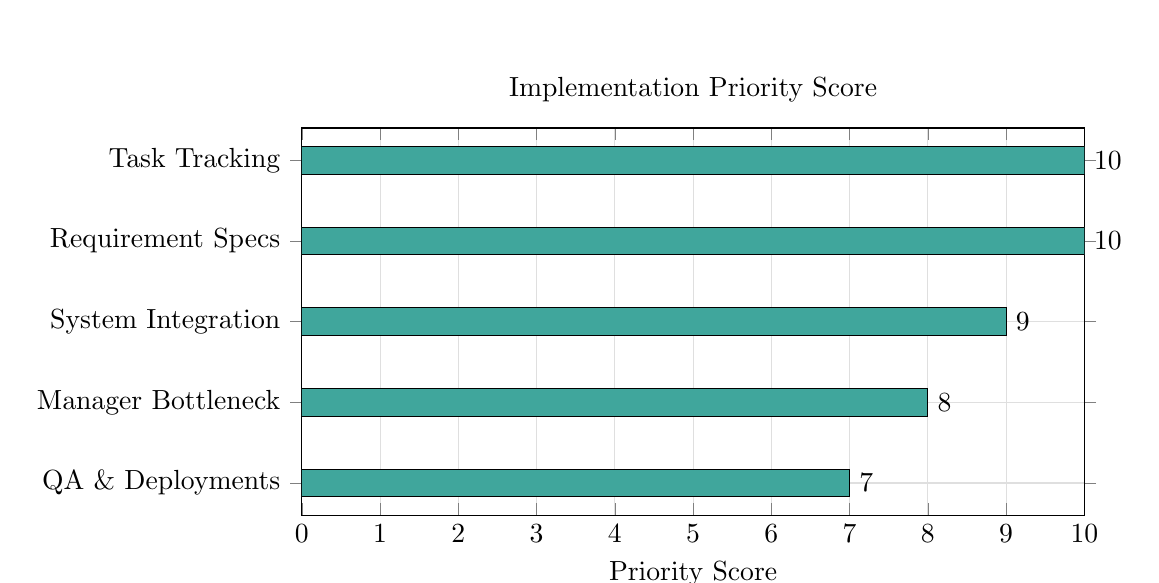
\begin{tikzpicture}
\begin{axis}[
    xbar,
    width=0.95\textwidth,
    height=6.5cm,
    xmin=0,
    xmax=10,
    xlabel={Priority Score},
    symbolic y coords={
        QA \& Deployments,
        Manager Bottleneck,
        System Integration,
        Requirement Specs,
        Task Tracking
    },
    ytick=data,
    nodes near coords,
    grid=major,
    major grid style={draw=gray!25},
    title={Implementation Priority Score}
]
\addplot[fill=accent!75] coordinates {
    (7,{QA \& Deployments})
    (8,{Manager Bottleneck})
    (9,{System Integration})
    (10,{Requirement Specs})
    (10,{Task Tracking})
};
\end{axis}
\end{tikzpicture}
\caption{Priority Ranking of Proposed Improvements}
\end{figure}

\section{Conclusion}

The initial feasibility study ensures that the top five critical operational boundaries holding back NextStepBD's scalability can be overcome reasonably. The company does not need heavy capital injections; rather, it requires an overhaul of its organizational workflow and engineering principles.

The most urgent changes are the establishment of a centralized task tracking system and formalizing requirement gathering before writing any code. Addressing these first provides an immediate return on efficiency. Following these, solving the PM bottleneck and cementing basic CI/CD testing systems will ensure quality isn't sacrificed for speed. Overall, standardizing these internal pipelines is highly feasible and sets the technical and cultural foundation required for the organization's next stage of growth.

\end{document}
